\documentclass[a4paper]{article}
\usepackage[left=3cm,right=3cm,top=2cm,bottom=2cm]{geometry} % page settings
\usepackage{enumerate}
\usepackage{hyperref}
\usepackage{graphicx}
\usepackage{amsfonts}
\usepackage{amsthm}
\usepackage{mathtools}
\usepackage{titlesec}
\usepackage{polski}
\usepackage{tikz}
\usepackage[utf8]{inputenc}
\DeclarePairedDelimiter\ceil{\lceil}{\rceil}
\DeclarePairedDelimiter\floor{\lfloor}{\rfloor}
\DeclarePairedDelimiter\set{\lbrace}{\rbrace}
\newcommand{\rpm}{\raisebox{.2ex}{$\scriptstyle\pm$}}


\def\checkmark{\tikz\fill[scale=0.3](0,.35) -- (.25,0) -- (1,.7) -- (.25,.15) -- cycle;} 

\titlespacing*{\subsection}
{0ex}{10ex}{3ex}

\title{Lista 8}
\author{Kamil Matuszewski}
\date{\today}

\begin{document}

\maketitle
\setlength{\parindent}{0.5ex}
\setlength{\parskip}{1.5ex}
\newcommand{\R}{\mathbb{R}}
\newcommand{\N}{\mathbb{N}}


\begin{center}
\begin{tabular}{|c *{9}{|c} |c|}\hline
1 & 2 & 3 & 4 & 5 & 6 & 7 & 8 & 9 & 10 & 11\\
\hline 
 & &\checkmark &\checkmark &\checkmark &\checkmark &\checkmark &\checkmark & & & \\
\hline
\end{tabular}\\
\end{center}
\subsection*{Zadanie 1}
Pociągi do miejscowości A odjeżdżają co 10 minut, rozpoczynając od 7.00. Pociągi do miejscowości B odjeżdżają co 15 minut, rozpoczynając od 7.05. Pasażer $P_1$ przychodzi na stację w czasie o rozkładzie jednostajnym pomiędzy 7.00 a 8.00; pasażer $P_2$ przychodzi na stację w czasie o rozkładzie jednostajnym pomiędzy 7.10 a 8.10. Jakie jest ppb, że pasażer $P_1$ dojedzie do A? Jakie jest ppb, że pasażer $P_2$ dojedzie do A?

Na to zadanie chyba można patrzeć tak:\\
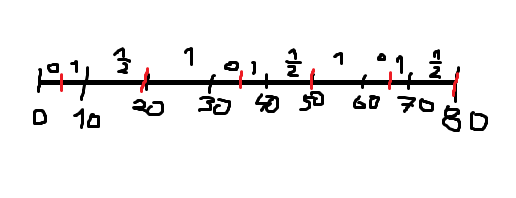
\includegraphics[scale=0.7]{z1l8.png}\\
Nad osią napisałem jakie są prawdopodobieństwa trafienia na pociąg A. Jeśli w tym czasie pierwszy przyjedzie pociąg do B, to szansa jest zero. Jeśli przyjadą dwa pociągi, szansa jest $\frac{1}{2}$. Patrzymy na $7:00$ jako na punkt 0, a pasażer przychodzi o pełnych minutach. To oznacza, że skoro pasażer 1 może przyjść do $8:00$, to przedział to $[0,60]$. Stąd, to co musimy policzyć, to sumę całek z przemnożonym prawdopodobieństwem. Skoro rozkład jest jednostajny, gęstość jest równa $\frac{1}{60}$, możemy więc wyciągnąć $\frac{1}{60}$ przed nawias. Mamy więc:
$$\frac{1}{60}\left( \int_{5}^{10}1\ dx+ \frac{1}{2} \int_{10}^{20} 1\ dx + \int_{20}^{30}1\ dx + \int_{35}^{40} 1\ dx + \frac{1}{2} \int_{40}^{50} 1\ dx +\int_{50}^{60} 1\ dx \right)=$$
$$=\frac{1}{60} \left( 5 + 5 + 10 + 5 + 5 + 10 \right) = \frac{2}{3} $$
Podobnie dla pasażera B, tylko tym razem przedział to $[10,70]$. Wartości także wyczytujemy z rysunku. Możemy zauważyć, że to będzie dokładnie to samo, bo odpadnie nam $\int_{5}^{10} 1\ dx$ a dojdzie $\int_{65}^{70} 1\ dx $ a poza tym będziemy mieć to samo, stąd prawdopodobieństwo także wyniesie $\frac{2}{3}$

Uwaga, nie jestem pewien czy rozwiązanie jest poprawne.

\subsection*{Zadanie 3,4}
Niezależne zmienne $X_1$ i $X_2$ mają rozkład $U[0,1]$. Niech $Y_1=2X_1+2X_2$ a $Y_2=X_1X_2$.
\begin{itemize}
\item Wyznacz wartość oczekiwaną $Y_1$:\\
$$E(Y_1)=E(2X_1+2X_2)=E(2X_1)+E(2X_2)=2\int_1^2 x_1\ dx_1 + 2\int_1^2 x_2\ dx_2 = 3+3=6$$
\item Wyznacz wartość oczekiwaną $Y_2$:\\
$$E(Y_2)=E(X_1X_2)=\int_1^2 \int_1^2 x_1 x_2\ dx_1\ dx_2 = \frac{3}{2}\cdot \frac{3}{2} = \frac{9}{4} $$
\item Wyznacz wariancje $Y_1$
$$V(Y_1)=E(Y_1^2)-E(Y_1)^2 = E(4X_1^2 + 8X_1X_2 + 4X_2^2) - 36 = 4E(X_1^2)+8E(X_1X_2)+4E(X_2^2) - 36$$
$$E(X_1^2)=E(X_2^2)=\int_1^2 x_1^2 \ dx_1 = \frac{7}{3} $$
$$V(Y_1)=4\frac{14}{3}-36+8E(Y_2)=4\frac{14}{3}-36+8\frac{9}{4}=\frac{2}{3}$$
\item Wyznacz wariancje $Y_2$
$$V(Y_2) = E(Y_2^2)-E(Y_2)^2 = E(X_1^2X_2^2)-\frac{81}{16} = \int_1^2 x_1^2 \int_1^2 x_2^2\ dx_2 \ dx_1 = \frac{49}{9}-\frac{81}{16}=\frac{55}{144}$$
\item Wyznacz współczynnik korelacji $Y_1$ i $Y_2$.
$$p=\frac{E[(Y_1 - EY_1)(Y_2 - EY_2)]}{\sqrt{V(Y_1)V(Y_2)}}=\frac{E[(2X_1+2X_2 - 6)(X_1X_2 - \frac{9}{4})]}{\sqrt{\frac{55}{216}}} = \frac{1}{2\sqrt{\frac{55}{216}}}=\frac{3\sqrt{330}}{55}$$

\end{itemize}

\subsection*{Zadanie 5}
Ze zbioru $n$ elementowego losujemy jakiś podzbiór. Niech zmienna losowa $X$ oznacza liczbę elementów wylosowanego podzbioru. Znajdź $E(X)$.

Mamy $n$ elementowy zbiór, więc $2^n$ podzbiorów, bez zbioru pustego mamy $2^{n}-1$\\ 
Prawdopodobieństwo wylosowania każdego zbioru jest równe $\frac{1}{2^n-1}$\\
Wtedy:\\
$$E(X)=\sum_{A\in P(S)}|A| \frac{1}{2^n-1} = \frac{1}{2^n-1}\sum_{A\in P(S)}|A|$$
Gdzie $P(S)$ oznacza moc podzbioru. Zadanie sprowadzamy więc do wyliczenia sumy po mocach wszystkich podzbiorów.\\
Jak wygląda ta suma? Wiemy, że w zbiorze $n$ elementowym liczba podzbiorów $i$ elementowych to ${n \choose i}$ (z dyskretnej). Innymi słowy ta suma to:
$$\sum_{i=0}^n {n \choose i} i = n2^{n-1}$$
Co pokażę:
$$f(x)=(1+x)^n = \sum_{i=0}^n {n \choose i} x^i \Rightarrow f'(x)=n(1+x)^{n-1}=\sum_{i=0}^n i{n \choose i} x^{i-1}$$
$$f'(1)=n2^{n-1}=\sum_{i=0}^n i{n \choose i} $$

Wracając do oryginalnego zadania, mamy:
$$E(X)=\frac{1}{2^n-1}\sum_{A\in P(S)}|A|=\frac{1}{2^n-1}\sum_{i=0}^n {n \choose i} i = \frac{1}{2^n-1}n2^{n-1}=\frac{n}{2^{1-n}(2^n-1)}=\frac{n}{2-2^{1-n}}=\frac{n}{2-(0.5)^{n-1}} $$
Co jest naszą odpowiedzią.

\subsection*{Zadanie 6}

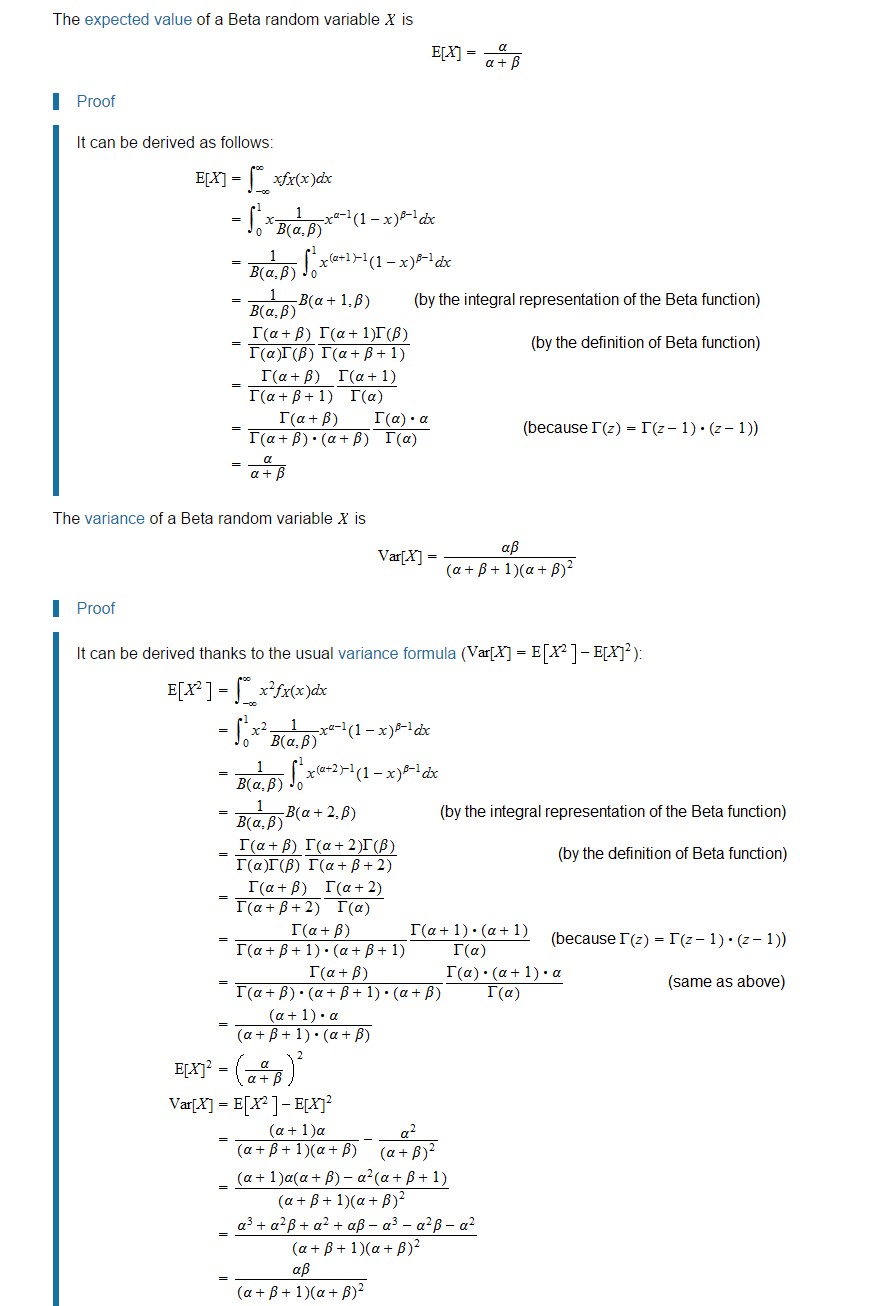
\includegraphics[scale=0.7]{z6l8}\\

\subsection*{Zadanie 7}
Metodą NW znaleźć estymator parametru $\lambda$ w rozkładzie Poissona.

Zadanie to jest identyczne jak zadanie $7$ z poprzedniej listy.

\subsection*{Zadanie 8}
Metodą NW znaleźć estymator parametru $p$ rozkładu Bernoulliego.

$$f(n,p)=p^n(1-p)^{1-n}$$
$$L=\prod\limits_{i=0}^n P(x_i, p) = p^k(1-p)^{n-k}$$
Gdzie k to liczba sukcesów ($x_i = 1$). 
$$\log{L}=k \log{p} + (n-k) log{(1-p)}$$
$$\frac{d\log{L}}{dp} = \frac{k-np}{p-p^2}$$
Przyrównajmy do 0:
$$\frac{k-np}{p-p^2} = 0 \Rightarrow p=\frac{k}{n}$$



\end{document}
